\documentclass{article}

\usepackage{fancyhdr}
\usepackage{extramarks}
\usepackage{amsmath}
\usepackage{amsthm}
\usepackage{amsfonts}
\usepackage{tikz}
\usepackage[plain]{algorithm}
\usepackage{algpseudocode}
\usepackage[]{mcode}
\usepackage{graphicx}
\usepackage{epstopdf}

\usetikzlibrary{automata,positioning}

%
% Basic Document Settings
%

\topmargin=-0.45in
\evensidemargin=0in
\oddsidemargin=0in
\textwidth=6.5in
\textheight=9.0in
\headsep=0.25in

\linespread{1.1}

\pagestyle{fancy}
\lhead{\hmwkAuthorName}
\chead{\hmwkClass\ (\hmwkClassInstructor\ \hmwkClassTime): \hmwkTitle}
\rhead{\firstxmark}
\lfoot{\lastxmark}
\cfoot{\thepage}

\renewcommand\headrulewidth{0.4pt}
\renewcommand\footrulewidth{0.4pt}

\setlength\parindent{0pt}

%
% Create Problem Sections
%

\newcommand{\enterProblemHeader}[1]{
    \nobreak\extramarks{}{Problem \arabic{#1} continued on next page\ldots}\nobreak{}
    \nobreak\extramarks{Problem \arabic{#1} (continued)}{Problem \arabic{#1} continued on next page\ldots}\nobreak{}
}

\newcommand{\exitProblemHeader}[1]{
    \nobreak\extramarks{Problem \arabic{#1} (continued)}{Problem \arabic{#1} continued on next page\ldots}\nobreak{}
    \stepcounter{#1}
    \nobreak\extramarks{Problem \arabic{#1}}{}\nobreak{}
}

\setcounter{secnumdepth}{0}
\newcounter{partCounter}
\newcounter{homeworkProblemCounter}
\setcounter{homeworkProblemCounter}{1}
\nobreak\extramarks{Problem \arabic{homeworkProblemCounter}}{}\nobreak{}

%
% Homework Problem Environment
%
% This environment takes an optional argument. When given, it will adjust the
% problem counter. This is useful for when the problems given for your
% assignment aren't sequential. See the last 3 problems of this template for an
% example.
%
\newenvironment{homeworkProblem}[1][-1]{
    \ifnum#1>0
        \setcounter{homeworkProblemCounter}{#1}
    \fi
    \section{Problem \arabic{homeworkProblemCounter}}
    \setcounter{partCounter}{1}
    \enterProblemHeader{homeworkProblemCounter}
}{
    \exitProblemHeader{homeworkProblemCounter}
}

%
% Homework Details
%   - Title
%   - Due date
%   - Class
%   - Section/Time
%   - Instructor
%   - Author
%

\newcommand{\hmwkTitle}{Tutorial\ 1}
\newcommand{\hmwkDueDate}{March 10, 2017}
\newcommand{\hmwkClass}{Digital Signal Processing}
\newcommand{\hmwkClassTime}{}
\newcommand{\hmwkClassInstructor}{Friso DeBoer}
\newcommand{\hmwkAuthorName}{S.Reynolds (262538)}

%
% Title Page
%

\title{
    \vspace{2in}
    \textmd{\textbf{\hmwkClass:\ \hmwkTitle}}\\
    \normalsize\vspace{0.1in}\small{Due\ on\ \hmwkDueDate\ at 3:00pm}\\
    \vspace{0.1in}\large{\textit{\hmwkClassInstructor\ \hmwkClassTime}}
    \vspace{3in}
}

\author{\textbf{\hmwkAuthorName}}
\date{}

\renewcommand{\part}[1]{\textbf{\large Part \Alph{partCounter}}\stepcounter{partCounter}\\}

%
% Various Helper Commands
%

% Useful for algorithms
\newcommand{\alg}[1]{\textsc{\bfseries \footnotesize #1}}

% For derivatives
\newcommand{\deriv}[1]{\frac{\mathrm{d}}{\mathrm{d}x} (#1)}

% For partial derivatives
\newcommand{\pderiv}[2]{\frac{\partial}{\partial #1} (#2)}

% Integral dx
\newcommand{\dx}{\mathrm{d}x}

% Alias for the Solution section header
\newcommand{\solution}{\textbf{\large Solution}}

% Probability commands: Expectation, Variance, Covariance, Bias
\newcommand{\E}{\mathrm{E}}
\newcommand{\Var}{\mathrm{Var}}
\newcommand{\Cov}{\mathrm{Cov}}
\newcommand{\Bias}{\mathrm{Bias}}

\graphicspath{{../Images/}}

\begin{document}

\maketitle

\pagebreak

\begin{homeworkProblem}

The code used to answer this question is as follows:

\begin{lstlisting}
	clear; clc;
	%%%%%%%%%%%%%%%%%% 2.1 Complex Numbers %%%%%%%%%%%%%%%%%%%%%%%%%%%%%%%
	
	% (a) We can define complex numbers z1 and z2 and plot them with zvect
	% and print them with zprint
	
	z1 = -1 +j*0.3;
	z2 = 0.8 + j*0.7;
	
	figure(1)
	title('Question 2.1 (a) Plot')
	zvect([z1 z2])
	zprint([z1 z2])
	
	% (b) Find the conjugate and inverse for z1 and z2
	
	z1_inv = 1/z1;
	z2_inv = 1/z2;
	
	z1_conj = conj(z1);
	z2_conj = conj(z2);
	
	figure(2)
	title('Question 2.1 (b) Plot')
	zvect([z1_inv z2_inv z1_conj z2_conj])
	zprint([z1_inv z2_inv z1_conj z2_conj])
	
	
	% (c) Compute z1 + z2 and plot. Use zcat to show the sum as vectors
	% head to tail and use zprint to display the result numerically.
	
	z_add = z1 + z2;
	
	figure(3)
	title('Question 2.1 (c) Plot')
	zvect([z_add])
	hold on
	zcat([z1 z2])
	zprint([z1 z2])
	
	% (d) Compute z1.z2 and z1/z2 and plot. Use zvect plot function to show
	% how the angles of z1 and z2 determine
	
	z_mult = z1*z2;
	z_div = z1/z2;
	
	figure(4)
	title('Question 2.1 (d) Plot')
	zvect([z_mult z_div])
	zprint([z_mult z_div])
\end{lstlisting}

\break

\textbf{2.1 Part A}\\
The output from MATLAB when entering the complex numbers was as follows:

\begin{verbatim}
	Z =     X    +     jY     Magnitude    Phase    Ph/pi   Ph(deg)
	          -1         0.3       1.044    2.850    0.907   163.30
	         0.8         0.7       1.063    0.719    0.229    41.19
\end{verbatim}

\begin{figure}[h]
	\centering
	\includegraphics[scale=0.5]{Q21a.eps}
	\caption{Plot of exercise 2.1 Part A}
\end{figure}

\textbf{2.1 Part B}\\
The output from MATLAB when entering the complex conjugates and inverse complex numbers was as follows:

\begin{verbatim}
	Z =     X    +     jY     Magnitude    Phase    Ph/pi   Ph(deg)
		     -0.9174     -0.2752      0.9578   -2.850   -0.907  -163.30
		       0.708     -0.6195      0.9407   -0.719   -0.229   -41.19
		          -1        -0.3       1.044   -2.850   -0.907  -163.30
		         0.8        -0.7       1.063   -0.719   -0.229   -41.19
\end{verbatim}

\begin{figure}[h]
	\centering
	\includegraphics[scale=0.5]{Q21b.eps}
	\caption{Plot of exercise 2.1 Part B}
\end{figure}

\newpage

\textbf{2.1 Part C}\\
The output from MATLAB for the addition of the two complex numbers was as follows:

\begin{verbatim}
	Z =     X    +     jY     Magnitude    Phase    Ph/pi   Ph(deg)
		          -1         0.3       1.044    2.850    0.907   163.30
		         0.8         0.7       1.063    0.719    0.229    41.19
\end{verbatim}

\begin{figure}[h]
	\centering
	\includegraphics[scale=0.5]{Q21c.eps}
	\caption{Plot of exercise 2.1 Part C}
\end{figure}


\textbf{2.1 Part D}\\
The output from MATLAB for the addition of the two complex numbers was as follows:

\begin{verbatim}
	Z =     X    +     jY     Magnitude    Phase    Ph/pi   Ph(deg)
		       -1.01       -0.46        1.11   -2.714   -0.864  -155.51
		     -0.5221      0.8319      0.9821    2.131    0.678   122.11
\end{verbatim}

\begin{figure}[h]
	\centering
	\includegraphics[scale=0.5]{Q21d.eps}
	\caption{Plot of exercise 2.1 Part D}
\end{figure}

\end{homeworkProblem}

\newpage

\begin{homeworkProblem}
The implementation of a systhesis function used to additively combine periodic signals based on their complex representation is as follows:

\begin{lstlisting}
function xx = sumcos(f, Z, fs, dur)
% SUMCOS Function to systhesise a sum of cosine waves
% Usage:
%   xx = sumcos(f, Z, fs, dur)
%   f = vector of frequencies
%   Z = vector of complex exponentials
%   fs = the sampling rate in Hz
%   dur = total time duration of signal
%
%   Note: f and Z must be the same length.
%       Z(1) corresponds to frequency f(1)
%       Z(2) corresponds to frequency f(2)
    
    % We need to set the sampling vector according to fs
    t_samp = 0:1/fs:dur;
    t_len = length(t_samp);
    xx = sum(real(repmat(Z',1,t_len).*exp(j*2*pi*f'*t_samp)),1);
end
\end{lstlisting}

\vspace{0.5cm}

The script used to test the function in MATLAB was as follows:

\begin{lstlisting}
clear; clc;
%%%%%%%%%%%%%%%%%% 2.2 Sinusoidal Synthesis %%%%%%%%%%%%%%%%%%%%%%%%%

% Script runs the function and prints the results

fs = 200000;
dur = 0.25;

t = 0:1/fs:dur;

xx1 = sumcos([20], [1], fs, dur);
figure(1)
plot(t,xx1)

xx2 = sumcos([20 40], [1 1/2], fs, dur);
figure(2)
plot(t,xx2)

xx3 = sumcos([20 40 60 80], [1 -1 1 -1], fs, dur);
figure(3)
plot(t,xx3)
\end{lstlisting}

\newpage

The plot from the test script can be seen in Figures 5, 6 and 7:

\begin{figure}[h]
	\begin{minipage}{.5\textwidth}
		\centering
		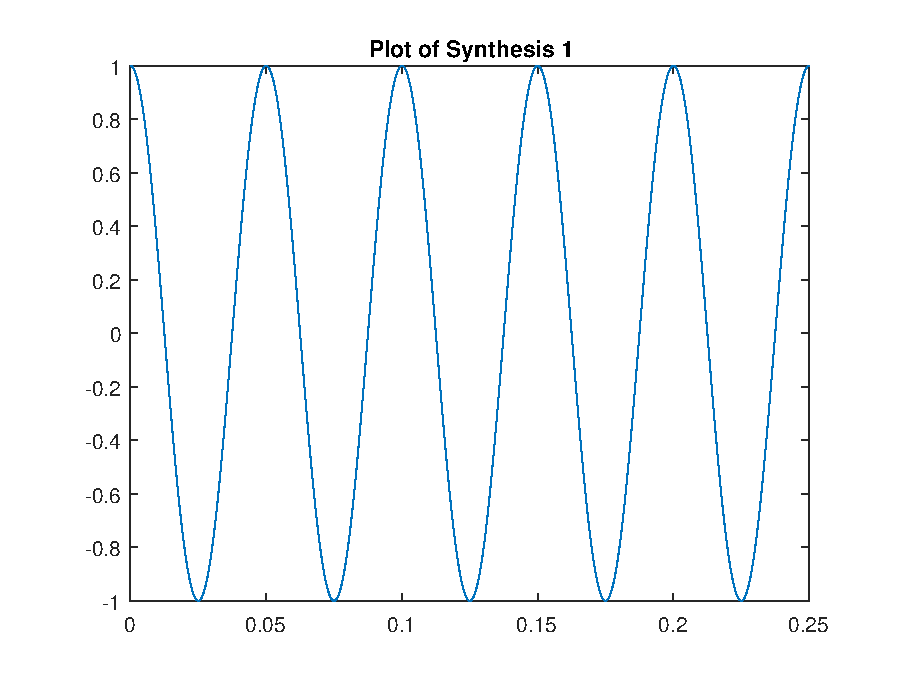
\includegraphics[scale=0.5]{Q22a.eps}
		\caption{Plot of exercise 2.2 Test 1}
	\end{minipage}
	\begin{minipage}{.5\textwidth}
		\centering
		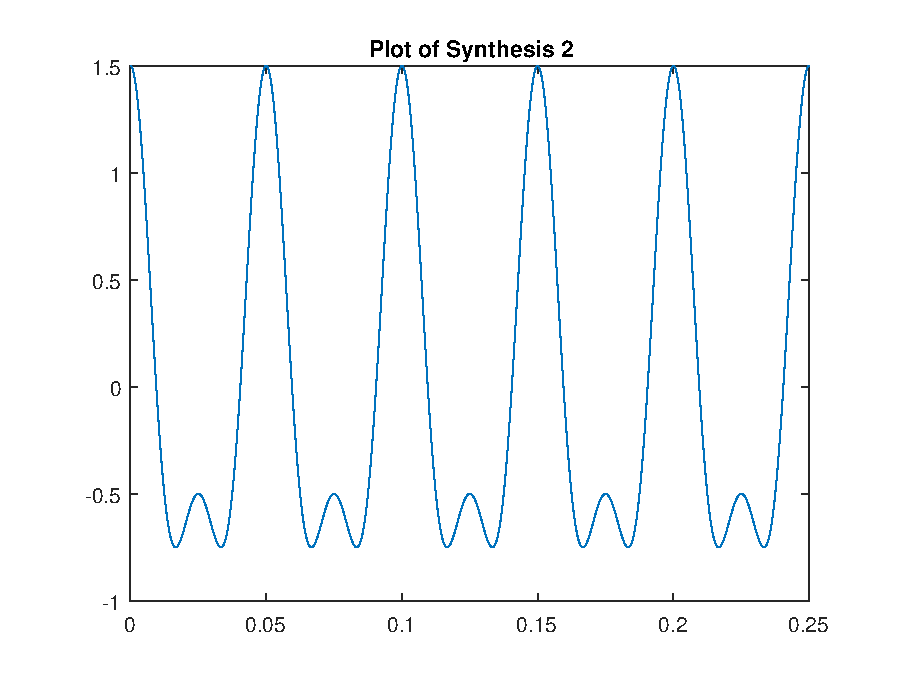
\includegraphics[scale=0.5]{Q22b.eps}
		\caption{Plot of exercise 2.2 Test 2}
	\end{minipage}
\end{figure}

\begin{figure}[h]
	\centering
	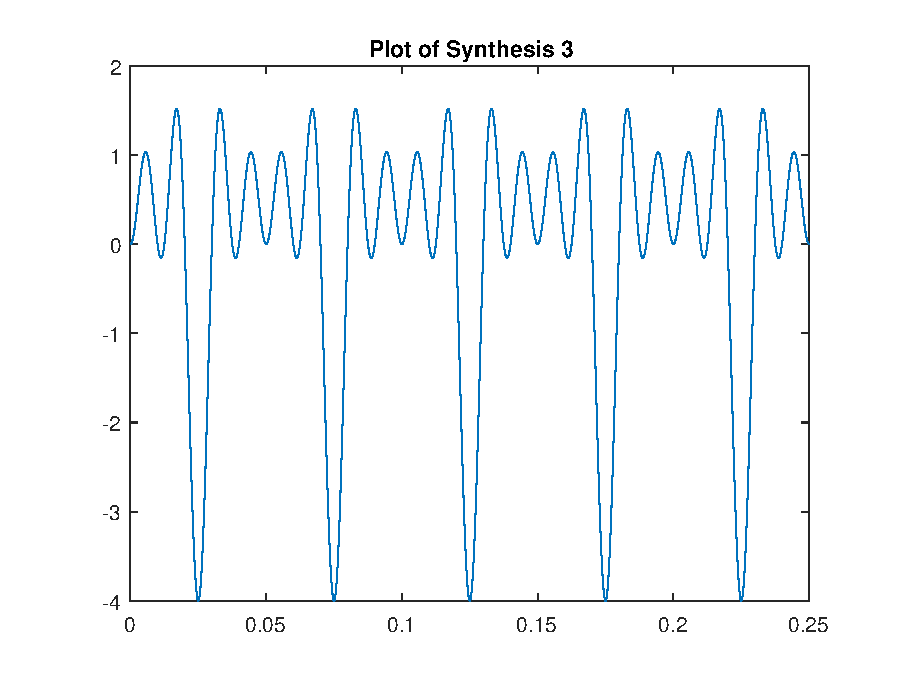
\includegraphics[scale=0.5]{Q22c.eps}
	\caption{Plot of exercise 2.2 Test 3}
\end{figure}

\end{homeworkProblem}

\newpage

\begin{homeworkProblem}
\textbf{3.1 Part A}\\
The following signal was generated in MATLAB for $A = 3$, $\phi = -0.4 \pi$, and $\omega_0 = 2 \pi \cdot (1250)$, over a range of 3 periods:
\begin{align}
	x(t) = A \cdot e^{j(\omega_0 t + \phi)} \nonumber
\end{align}

The MATLAB code used to implement it can be seen below:

\begin{lstlisting}
clear; clc;
%%%%%% 3.1 Representation of Sinusoids with Complex Exponentials %%%%%%

% Specify the parameters of the signal
A = 3;
phase = -0.4*pi;
f0 = 1250;
w0 = 2*pi*f0;

% Specify the discrete points the signal will be sampled at
T0 = 1/f0;
t = linspace(-T0,2*T0,2000);

% Create the signal
x = A*exp(j*(w0*t + phase));

subplot(2,1,1)
plot(t,real(x));
title('Real part of x(t)')

subplot(2,1,2)
plot(t,imag(x));
title('Imaginary part of x(t)')
\end{lstlisting}

\vspace{0.5cm}

\textbf{3.1 Part B}\\
Plots of the real and imaginary parts of the signal $x(t)$ can be seen in Figure 8:

\begin{figure}[h]
	\centering
	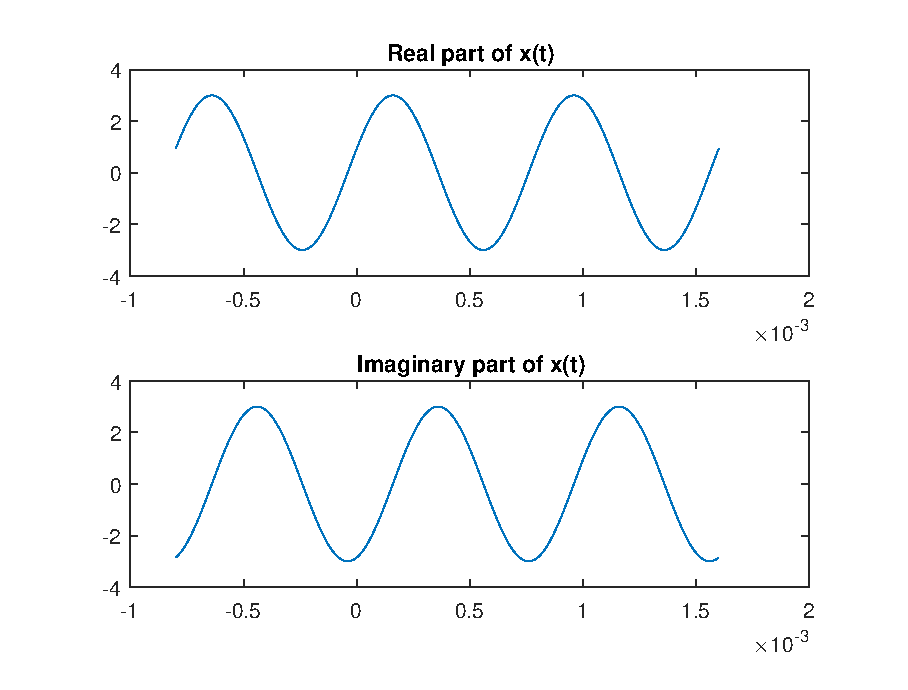
\includegraphics[scale=0.5]{Q31.eps}
	\caption{Plots of real and imaginary parts of complex signal}
\end{figure}

\end{homeworkProblem}

\begin{homeworkProblem}

The code used to implement this task in MATLAB is shown below:

\begin{lstlisting}
clear; clc;
%%%%%%% 3.2 Verify Addition of Sinusoids Using Complex Exponentials%%%%%%

% Specify parameters for plots
A = 5;
f0= 15;
T0 = 1/f0;

% Discretised sampling points for signals
t = linspace(-T0,2*T0,2000);

% Signals
x1 = A*cos(2*pi*f0*t + 0.5*pi); 
x2 = A*cos(2*pi*f0*t - 0.25*pi);
x3 = A*cos(2*pi*f0*t + 0.4*pi);
x4 = A*cos(2*pi*f0*t - 0.9*pi);

% Summation of signls
x5 = x1 + x2 + x3 + x4;

% Plots of signals
subplot(3,2,1)
plot(t,x1)
title('Plot of x1')
grid on

subplot(3,2,2)
plot(t,x2)
title('Plot of x2')
grid on

subplot(3,2,3)
plot(t,x3)
title('Plot of x3')
grid on

subplot(3,2,4)
plot(t,x4)
title('Plot of x4')
grid on

subplot(3,2,5)
plot(t,x5)
hold on
plot(t,A*cos(2*pi*f0*t))
title('Plot of x5')
grid on

% Complex arithmetic
Amp = [A A A A];
ph = [0.5 -0.25 0.4 -0.9]*pi;
Z = Amp.*exp(j*ph);
z1 = Z(1); z2 = Z(2); z3 = Z(3); z4 = Z(4);

% Add all the complex exponentials together
z5 = sum(Z);

zprint([z1 z2 z3 z4 z5])

figure(2)
zcat([z1 z2 z3 z4])
hold on
zvect([z5])
\end{lstlisting}

\vspace{0.5cm}

\textbf{3.2 Part A}\\

Plots were made for the following four signals:
\begin{align*}
	x_1(t) &= 5 \cdot cos(2 \pi (15)t + 0.5 \pi)\\
	x_2(t) &= 5 \cdot cos(2 \pi (15)t - 0.25 \pi)\\
	x_3(t) &= 5 \cdot cos(2 \pi (15)t + 0.4 \pi)\\
	x_4(t) &= 5 \cdot cos(2 \pi (15)t - 0.9 \pi)
\end{align*}

Plots can be seen in Figure 9:

\begin{figure}[h]
	\centering
	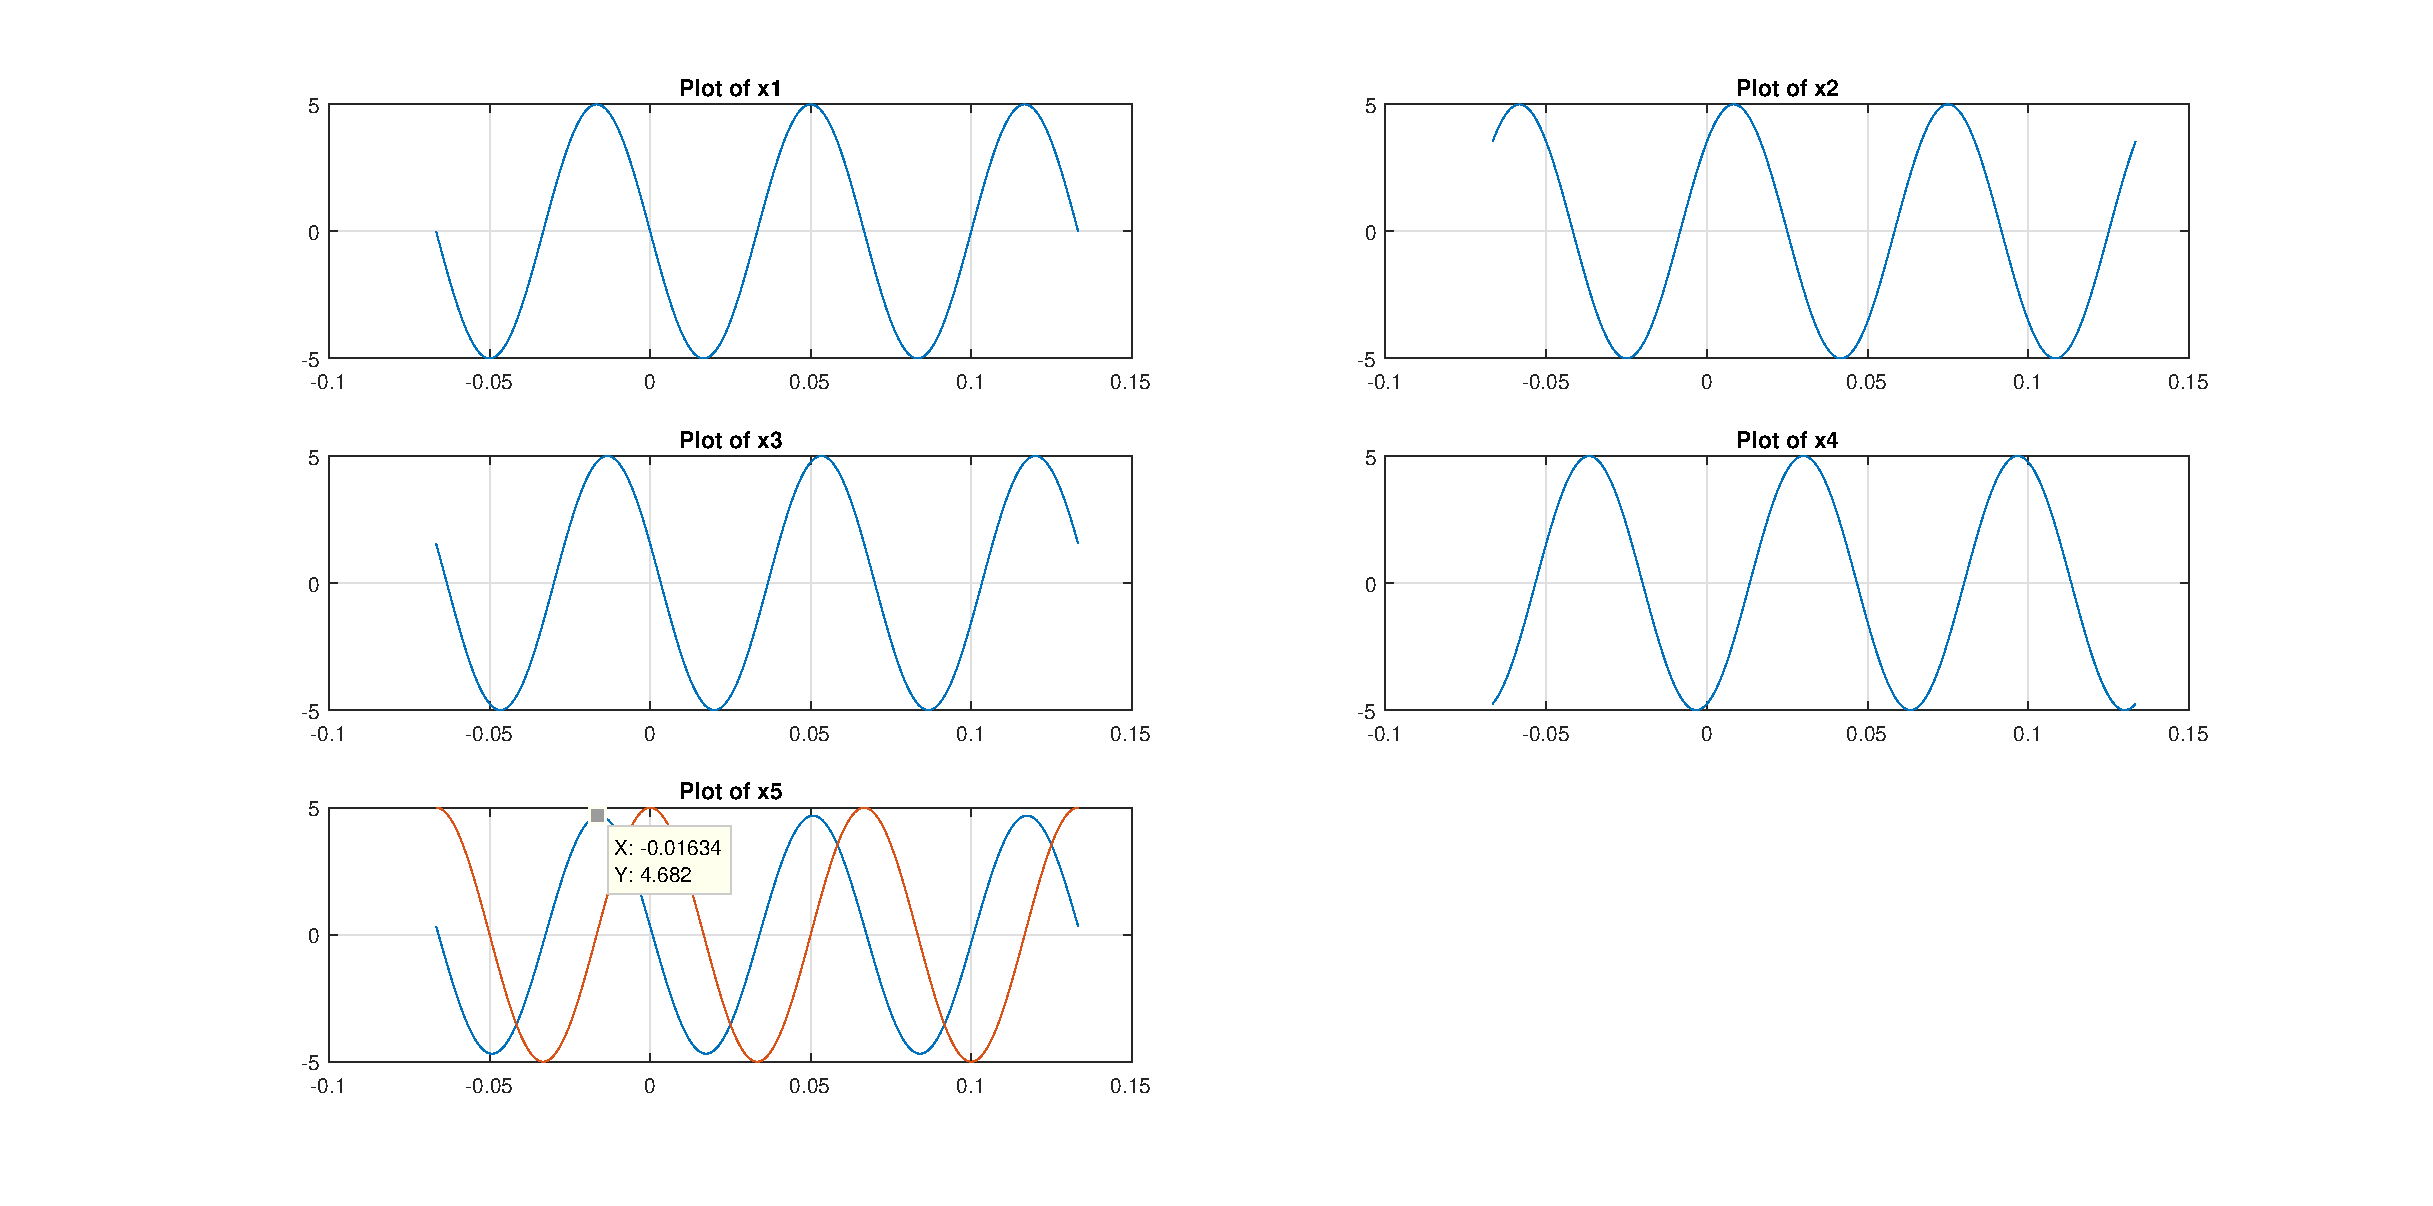
\includegraphics[scale=0.4]{Q32a.eps}
	\caption{Plots of $x_1(t)$ through to $x_5(t)$}
\end{figure}

\textbf{3.2 Part C}\\
A signal was created by adding the signals listed above:
\begin{align*}
	x_5(t) = x_1(t) + x_2(t) + x_3(t) + x_4(t)
\end{align*}

The plot can be seen in Figure \textbf{XX}

\vspace{0.5cm}

\textbf{3.2 Part D}\\
The magnitude of signal $x_5(t)$ is 4.682 and can be found visually inspecting the plot in Figure 9. The phase can be found by finding the time delay from a standard sinusoid, which was 0.01634 to the left. The phase is calculated as:

\begin{align*}
	\phi 	&= 360^o \cdot f_0 \cdot \delta t\\
			&= 360^o \cdot 15 \cdot 0.01634\\
			&= 88.24^o
\end{align*}

\vspace{0.5cm}

\textbf{3.2 Part E}\\
Using the MATLAB complex number print from the DSP First package, we can see the polar and Cartesian representations of the complex numbers $z_1$, $z_2$, $z_3$, $z_4$, and $z_5$, which relate to the signals $x_1(t)$ through to $x_5(t)$, respectively. The vales are displayed below:

\begin{verbatim}
Z =     X    +     jY     Magnitude    Phase    Ph/pi   Ph(deg)
   3.062e-16           5           5    1.571    0.500    90.00
       3.536      -3.536           5   -0.785   -0.250   -45.00
       1.545       4.755           5    1.257    0.400    72.00
      -4.755      -1.545           5   -2.827   -0.900  -162.00
      0.3253       4.675       4.686    1.501    0.478    86.02
\end{verbatim}

\vspace{0.5cm}

\textbf{3.2 Part F}\\
A plot of the addition of the 4 vectors, and the resultant vector can be seen in Figure 10 below.

\begin{figure}[h]
	\centering
	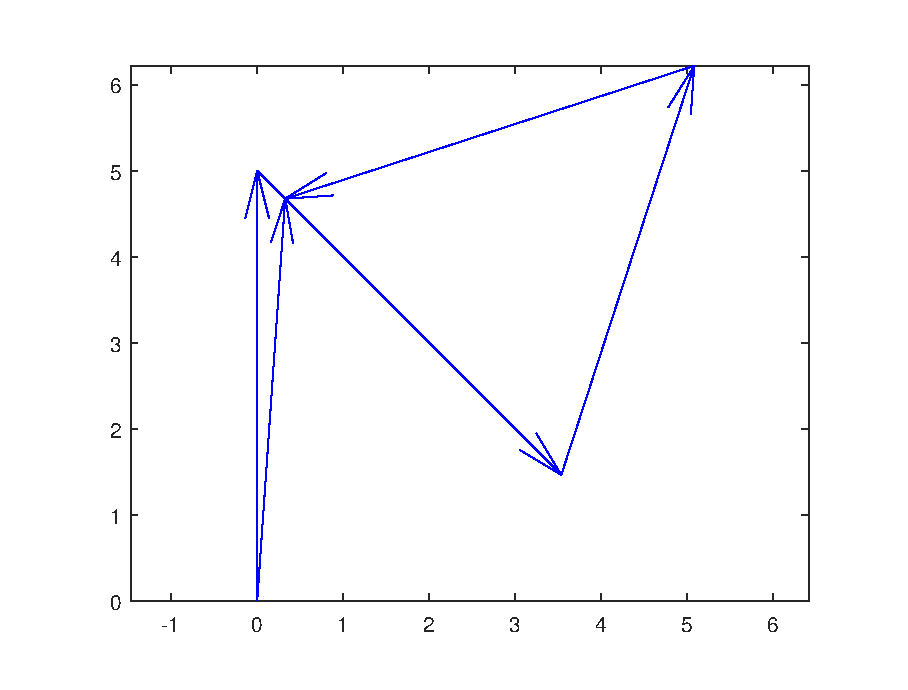
\includegraphics[scale=0.5]{Q32f.eps}
	\caption{Plot of vectors $z_1$ through $z_4$ added vector wise, and the resultant and vector $z_5$}
\end{figure}

\vspace{0.5cm}

\textbf{3.2 Part G}\\
The magnitude seen in part F matches the magnitude estimated from the plot in Figure 9. Similarly, the calculated phase matches the phase displayed in the MATLAB output.
\end{homeworkProblem}

\newpage

\begin{homeworkProblem}

\textbf{Part 4 A}\\
The code used to implement this task in MATLAB is shown below:

\begin{lstlisting}
	%%%%%%%%%%%%%%%%%%%%%%%%% 4 Periodic Waveforms %%%%%%%%%%%%%%%%%%%%%%%%%
	clear; clc;
	
	% fundamental frequency
	f0 = 25;
	Tmax = 1/f0;
	
	% sampling frequency
	fs = 20000;
	dur = 2*Tmax;
	t = 0:1/fs:dur;
	
	% Set up the vector of integers for the number of cosines
	N1 = 2*[0:4]+1; % 5 cosines
	N2 = 2*[0:9]+1; % 10 cosines
	N3 = 2*[0:24]+1; % 25 cosines
	
	% Create the frequency and Zk vectors for N = 5
	f1 = N1*f0;
	Z1 = j./N1;
	x1 = sumcos(f1,Z1,fs,dur); % Create plot for the N = 5
	subplot(3,1,1)
	plot(t,x1)
	title('5 Cosines')
	
	% Create the frequency and Zk vectors for N = 10
	f2 = N2*f0;
	Z2 = j./N2;
	x2 = sumcos(f2,Z2,fs,dur); % Create plot for the N = 10
	subplot(3,1,2)
	plot(t,x2)
	title('10 Cosines')
	
	% Create the frequency and Zk vectors for N = 25
	f3 = N3*f0;
	Z3 = j./N3;
	x3 = sumcos(f3,Z3,fs,dur); % Create plot for the N = 25
	subplot(3,1,3)
	plot(t,x3)
	title('25 Cosines')
\end{lstlisting}

\newpage

A plot of the three outputs of increasing number of sinusoidal curves in the synthesis can be seen in Figure 11 below.

\begin{figure}[h]
	\centering
	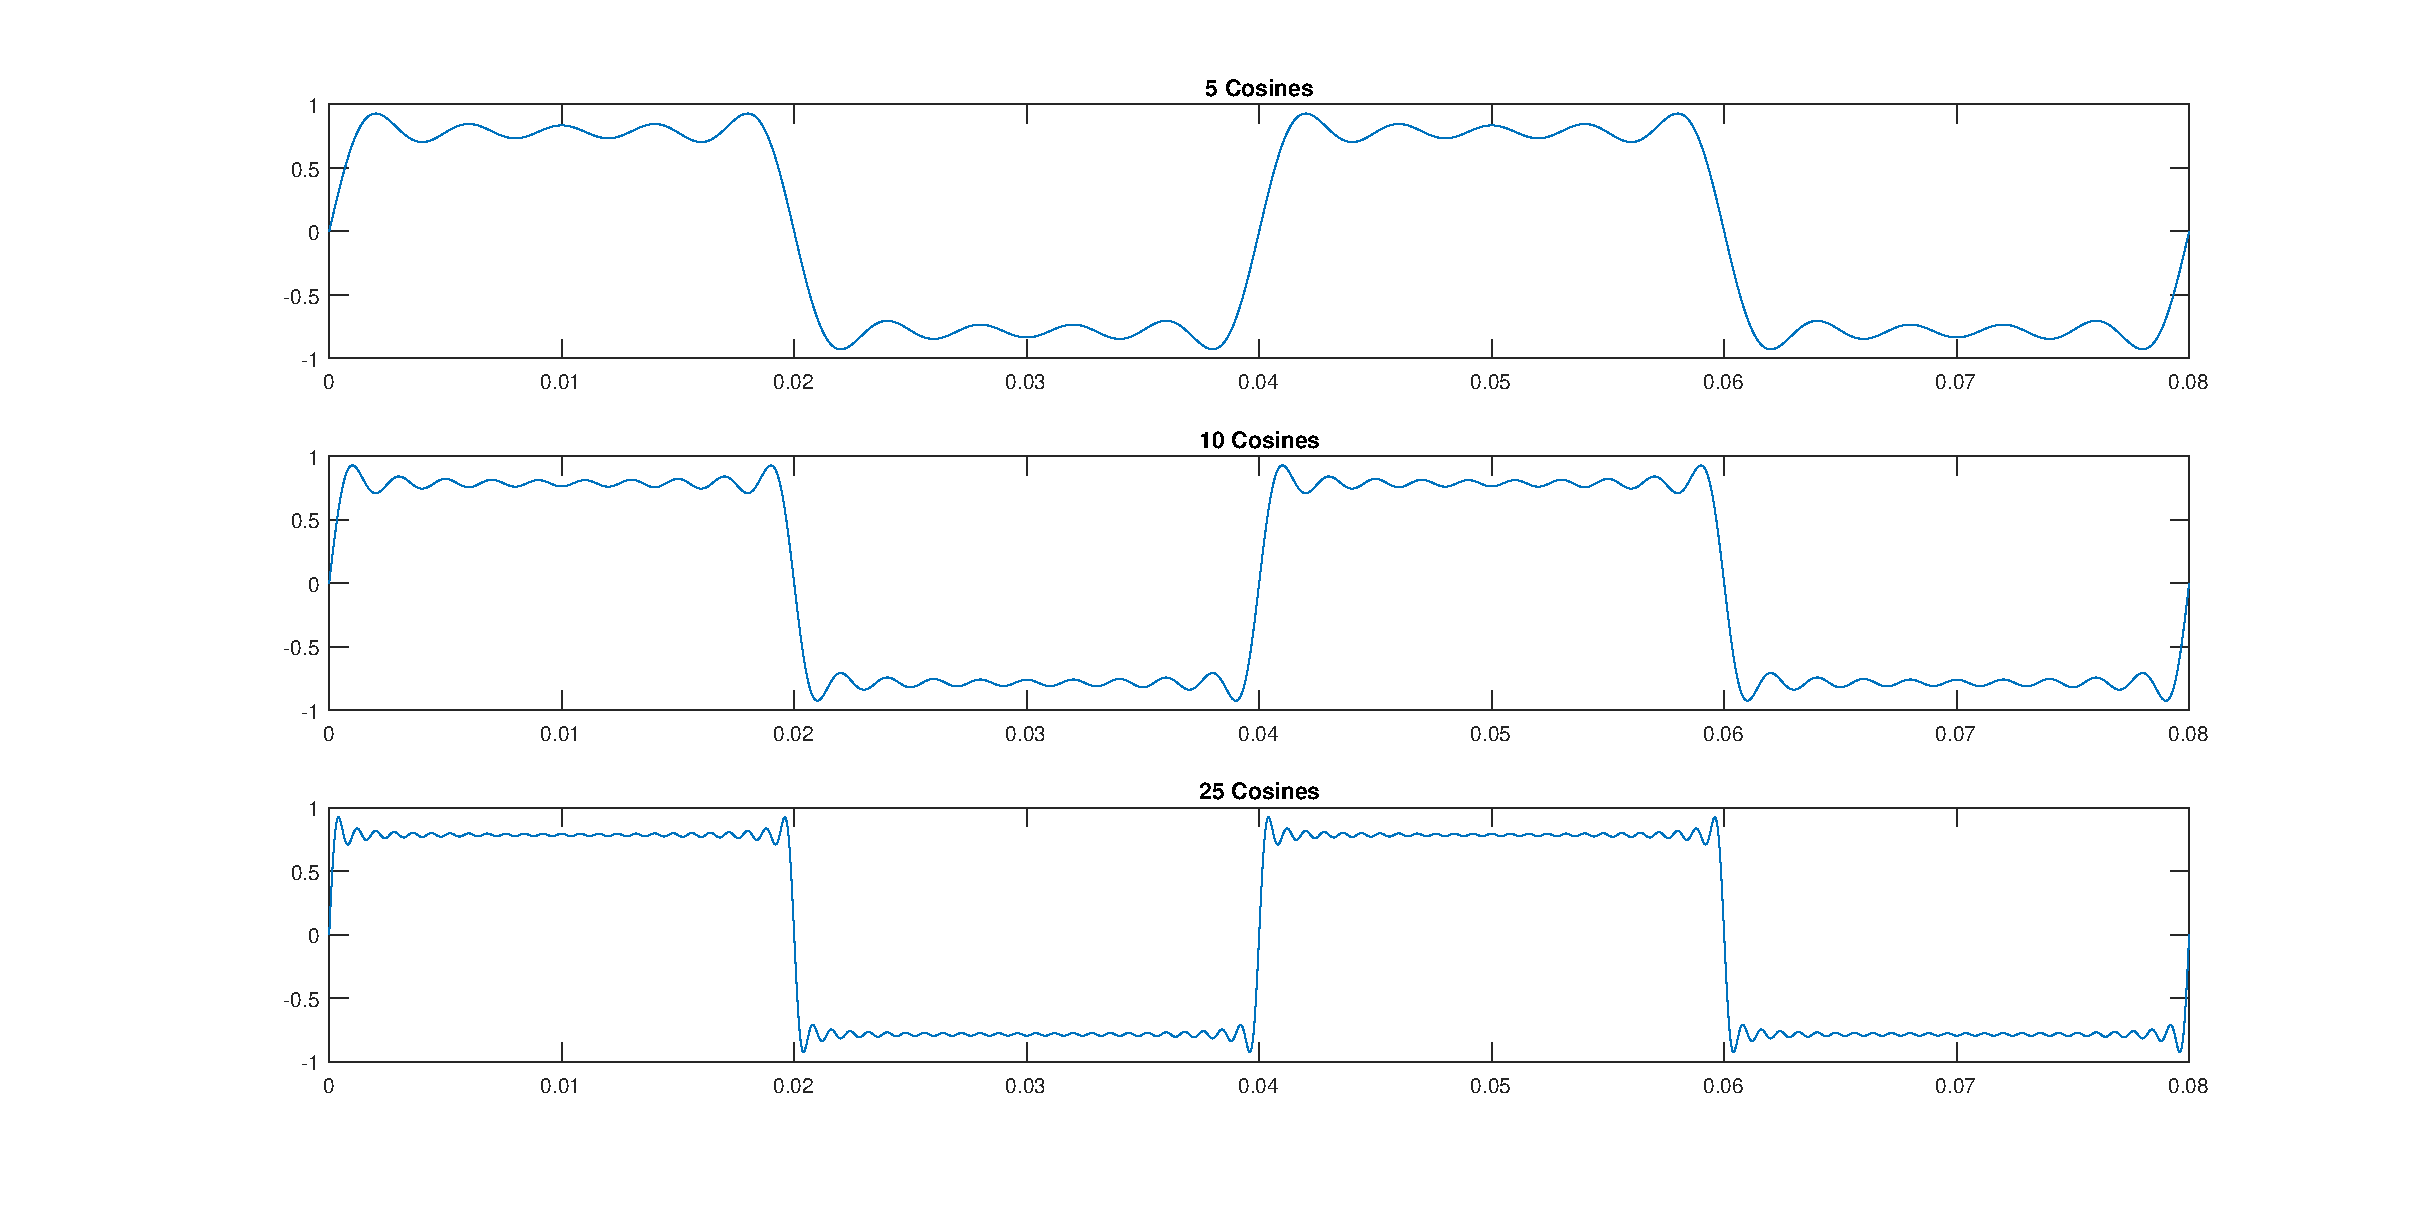
\includegraphics[scale=0.4]{Q4a.eps}
	\caption{Square wave estimation with increasing numbers of sinusoidal curves}
\end{figure}

The period of the waveform is approximately 0.04 seconds, which is the same as the fundamental period $T_0 = \frac{1}{f_0} = 0.04 $ seconds. As $N \rightarrow \infty$ we see that the synthesised curve approaches a square wave, however, this is only an approximation since the number of sinusoidal curves is always finite. As we increase the number of sinusoidal curves in the representation, we see an interesting phenomenon of transient peaks on the edges of the wave. This is known as Gibbs phenomenon.

\vspace{0.5cm}

\textbf{Part 4 B}\\
The code used to implement this task in MATLAB is shown below:
\begin{lstlisting}
%%%%%%%%%%%%%%%%%%%%%%%%% 4 Periodic Waveforms %%%%%%%%%%%%%%%%%%%%%%%%%
clear; clc;
% fundamental frequency
f0 = 1000;
Tmax = 1/f0;

% sampling frequency
fs = 20000;
dur = 2;
t = 0:1/fs:dur;
N_list = [0 1 2 3 4 9];

% Loop creates signal and plays the sound from the signal
for n = N_list
    N = 2*[0:n]+1;
    f = N*f0;
    Z = j./N;
    x = sumcos(f,Z,fs,dur);
    sound(x,fs)
    pause % to progress the code go to the terminal and hit enter
end
\end{lstlisting}

\textbf{Part 4 C}
The code used to implement this task in MATLAB is shown below:
\begin{lstlisting}
%%%%%%%%%%%%%%%%%%%%%%%%% 4 Periodic Waveforms %%%%%%%%%%%%%%%%%%%%%%%%%
clear; clc;

% fundamental frequency
f0 = 25;
Tmax = 1/f0;

% sampling frequency
fs = 20000;
dur = 2*Tmax;
t = 0:1/fs:dur;

% Set up the vector of integers for the number of cosines
N1 = [1:5]; % 5 cosines
N2 = [1:10]; % 10 cosines
N3 = [1:25]; % 25 cosines

% Create the frequency and Zk vectors for N = 5
f1 = N1*f0;
Z1 = (j*(-1).^N1)./(2*pi*N1);
x1 = sumcos(f1,Z1,fs,dur); % Create plot for the N = 5
subplot(3,1,1)
plot(t,x1)
title('5 Cosines')

% Create the frequency and Zk vectors for N = 10
f2 = N2*f0;
Z2 = (j*(-1).^N2)./(2*pi*N2);
x2 = sumcos(f2,Z2,fs,dur); % Create plot for the N = 10
subplot(3,1,2)
plot(t,x2)
title('10 Cosines')

% Create the frequency and Zk vectors for N = 25
f3 = N3*f0;
Z3 = (j*(-1).^N3)./(2*pi*N3);
x3 = sumcos(f3,Z3,fs,dur); % Create plot for the N = 25
subplot(3,1,3)
plot(t,x3)
title('25 Cosines')
\end{lstlisting}

\newpage

A plot of the three outputs of increasing number of sinusoidal curves in the synthesis can be seen in Figure 12 below.

\begin{figure}[h]
	\centering
	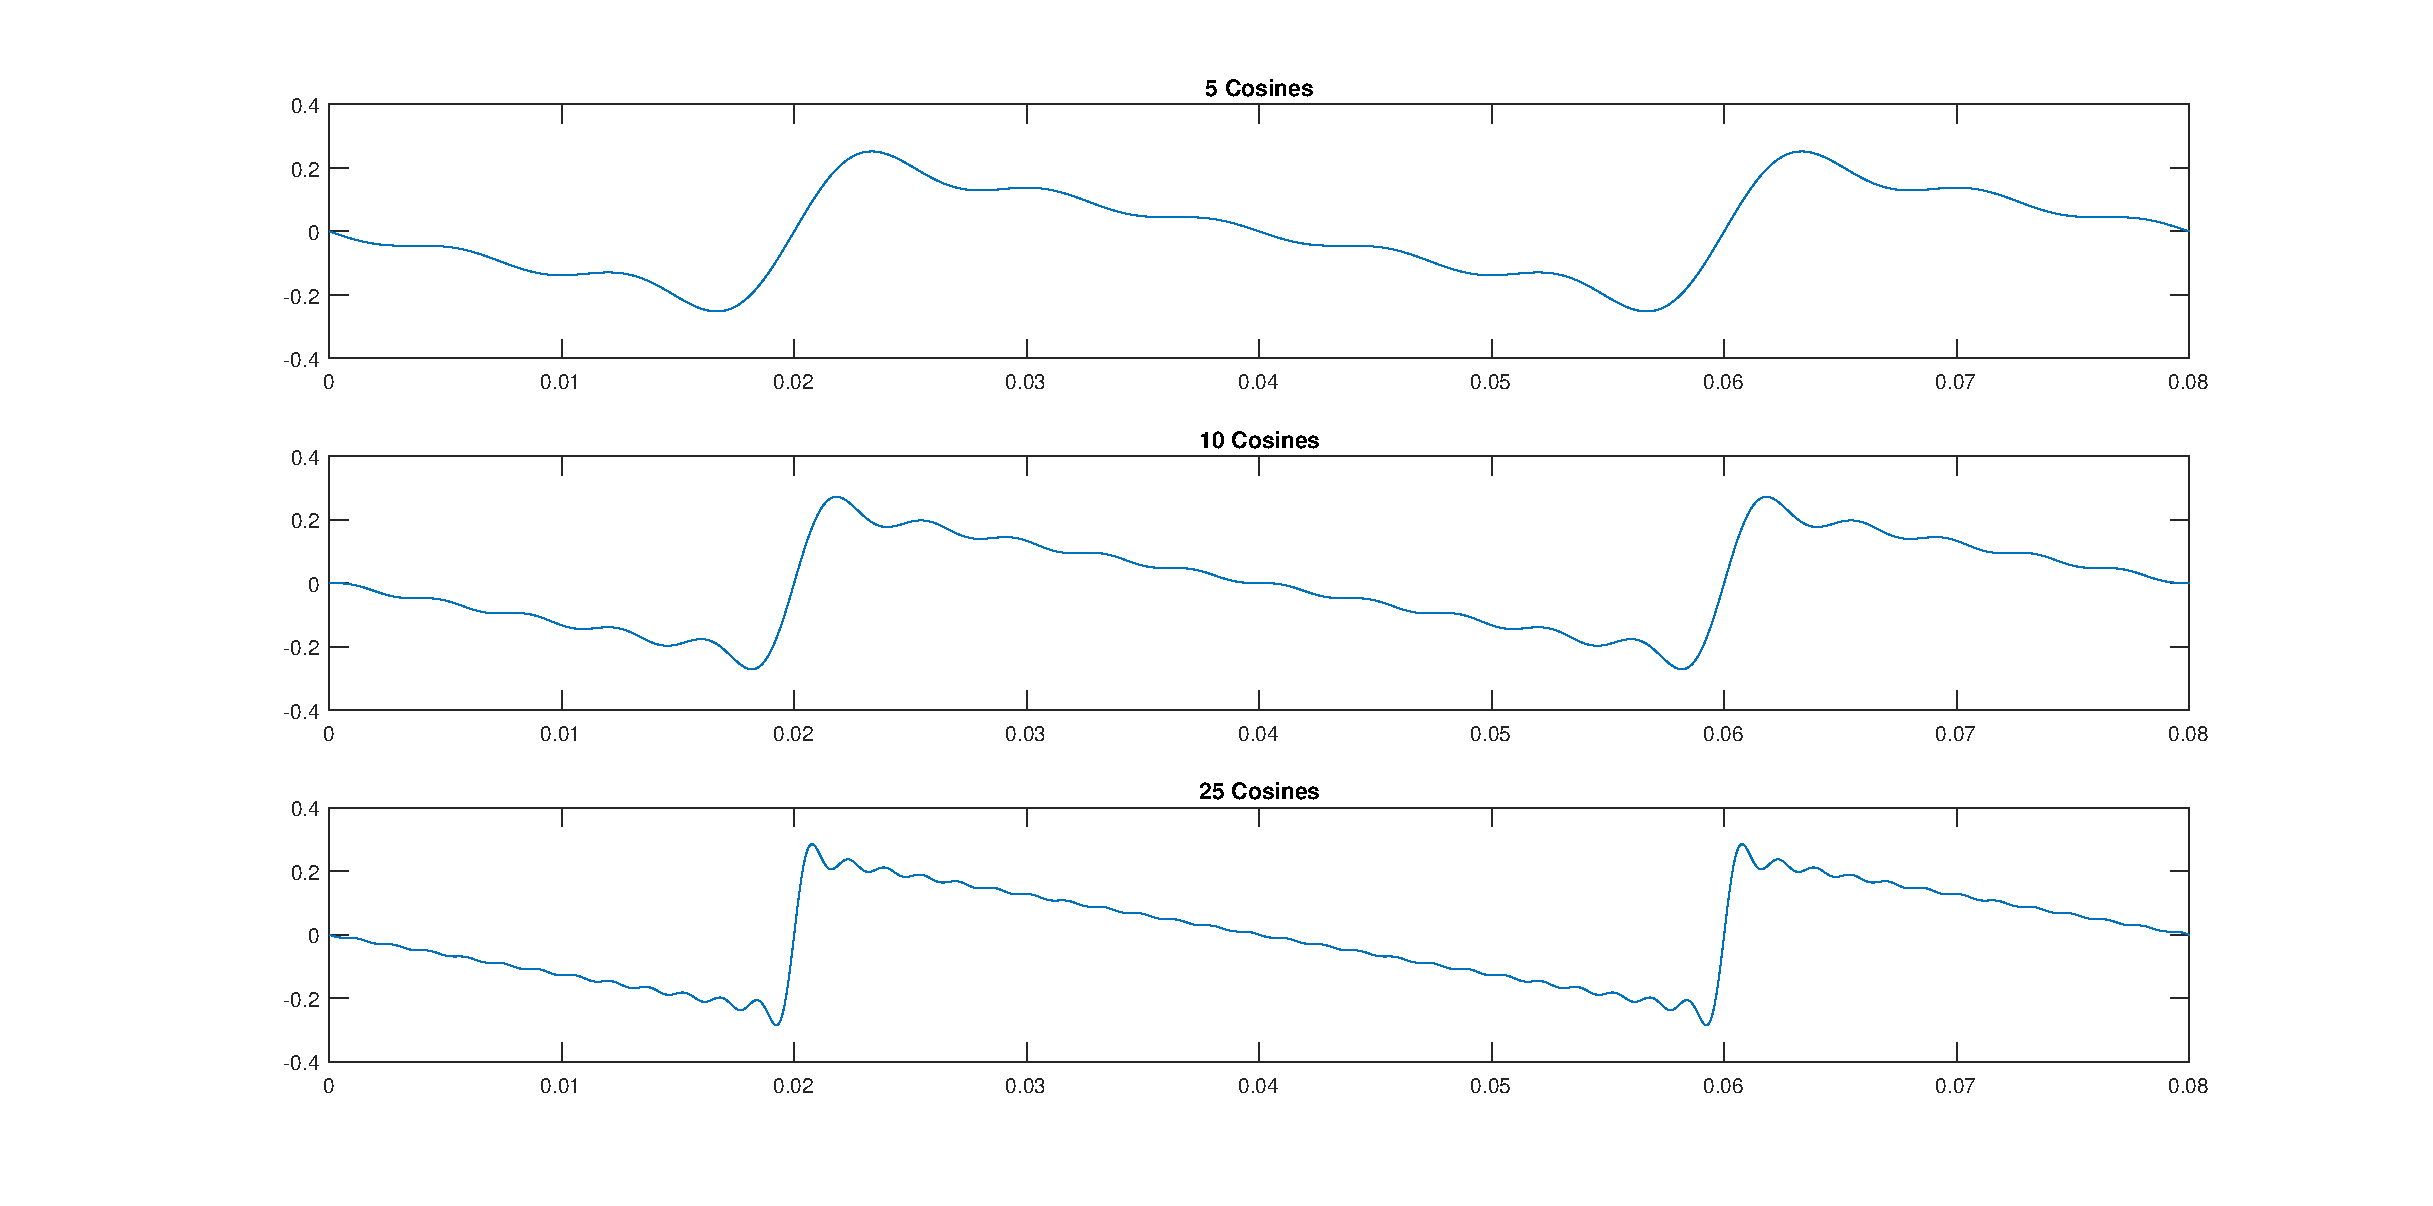
\includegraphics[scale=0.4]{Q4c.eps}
	\caption{Sawtooth wave estimation with increasing numbers of sinusoidal curves}
\end{figure}

The period of the waveform is approximately 0.04 seconds, which is the same as the fundamental period $T_0 = \frac{1}{f_0} = 0.04 $ seconds. As $N \rightarrow \infty$ we see that the synthesised curve approaches a sawtooth wave, however, this is only an approximation since the number of sinusoidal curves is always finite. As we increase the number of sinusoidal curves in the representation, we see an interesting phenomenon of transient peaks on the edges of the wave. This is known as Gibbs phenomenon.

\end{homeworkProblem}

\end{document}
